%!TEX root = ../main.tex
%%%%%%%%%%%%%%%%%%%%%%%%%%%%%%%%%%
% Links: https://www.geeksforgeeks.org/sort-array-wave-form-2/
%
% Difficulty: Medium Companies: 
%%%%%%%%%%%%%%%%%%%%%%%%%%%%%%%%%%

\chapter{Wave Array}
\label{ch:wave_array}
\section*{Introduction}
We are used to talking about sorting in terms of arranging items in either ascending or descending order, but in fact, sorting is simply the process of arranging items systematically according to a criterion that can be purely arbitrary.

The problem discussed in this Chapter concerns writing an algorithm for sorting the elements of a collection in an unusual way by placing them at even indices such that each is surrounded by either greater or smaller elements. For example, the collection: $\{1,3,-1,3,2,4\}$ is properly sorted on these terms whilst $\{1,3,-1,1,2,4\}$ is not.

This question often arises at first on-site interview stage for companies like \textit{Adobe}, and \textit{Google}, mostly  as it is not considered particularly difficult and should be solvable by writing just a few lines code. It can, however, prove challenging to get right the first time under pressure therefore, once a working draft of the solution is finished, our advice is to still take time to make sure the code is behaving as expected, especially in edge case scenarios.

\section{Problem statement}
\begin{exercise}
\label{ex:wave_array:statement}

Given an array $A$ of $n$ integers, arrange the numbers in a wave-like fashion. A valid wave array $X$ has its elements arranged in one of the two following ways:
	\begin{enumerate}
		\item  $x_0 \geq x_1 \leq x_2 \geq x_3 \leq  x_5 \geq \ldots$ where $x_{2i-1} \geq x_{2i} \leq x_{2i+1}$
		\item  $x_1 \leq x_2 \geq x_3 \leq x_4 \geq x_5 \leq \ldots$ where $x_{2i-1} \leq x_{2i} \geq x_{2i+1}$
	\end{enumerate}


	\begin{example}
		\hfill \\
		\label{ex:wave_array:example1}
		Given $A= \{10, 5, 6, 3, 2, 20, 100, 80\}$ the followings are all valid output (see Figure \ref{fig:wave_array:example1}):
		\begin{itemize}
			\item  \{20, 5, 10, 2, 80, 6, 100, 3\}
			\item  \{10, 5, 6, 2, 20, 3, 100, 80\}
		\end{itemize}
	\end{example}

	\begin{example}
		\hfill \\
		\label{ex:wave_array:example2}
		Given $A= \{20, 10, 8, 6, 4, 2\}$ the followings are all valid output (see Figure \ref{fig:wave_array:example1}):
		\begin{itemize}
			\item \{20, 8, 10, 4, 6, 2\}
			\item  \{10, 8, 20, 2, 6, 4\}
		\end{itemize}
		
	\end{example}

	\begin{example}
		\hfill \\
		\label{ex:wave_array:example3}
		Given $A= \{10,9,8,7,6,5,4,3,2,1\}$ the following is a output: $\{10, 8, 9, 6, 7, 4, 5, 2, 3, 0,
		1 \}$ (see Figure \ref{fig:wave_array:example1}).
		
	\end{example}
\end{exercise}

\begin{figure}
	\centering
	\begin{subfigure}[t]{0.80\textwidth}
		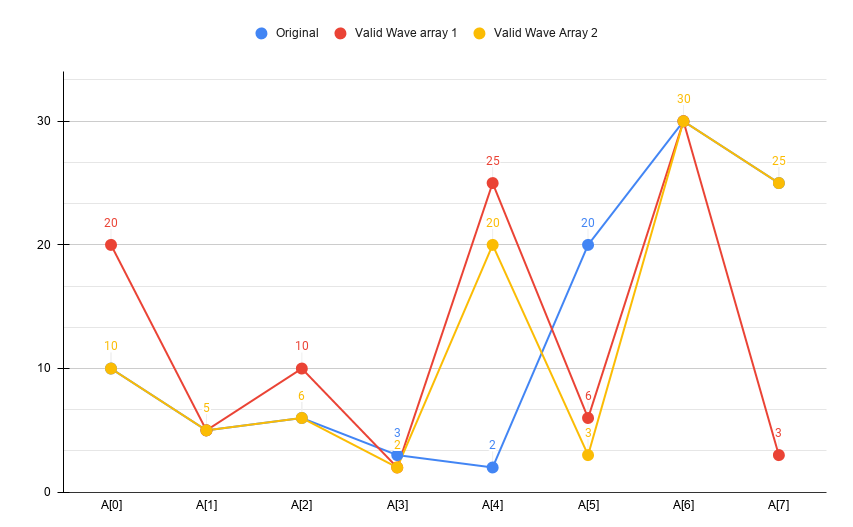
\includegraphics[width=1\linewidth]{sources/wave_array/images/example1.png}
		\caption{Input and solutions for Example \ref{ex:wave_array:example1}.}
		\label{fig:wave_array:example1}
	 \end{subfigure}
	\hfill
	\begin{subfigure}[t]{0.80\textwidth}
		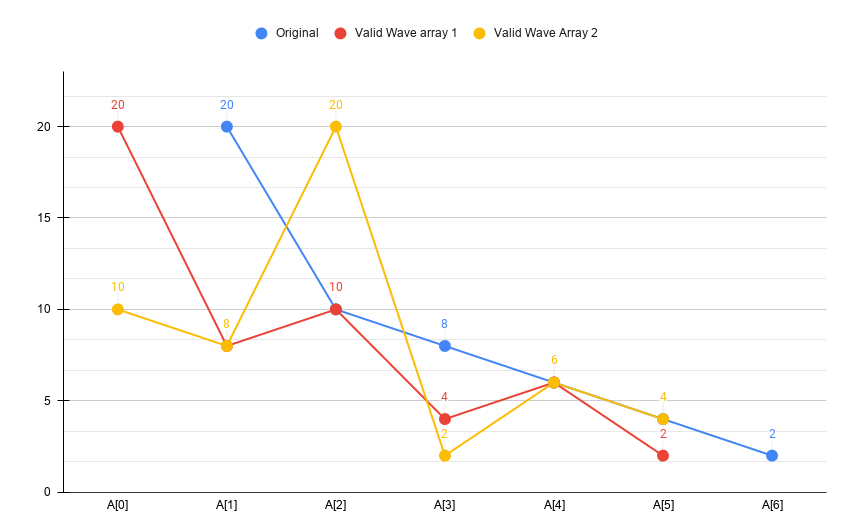
\includegraphics[width=1\linewidth]{sources/wave_array/images/example2.png}
		\caption{Input and solutions for Example \ref{ex:wave_array:example2}.}
		\label{fig:wave_array:example2}
	 \end{subfigure}
	 \hfill
	 \begin{subfigure}[t]{0.80\textwidth}
		 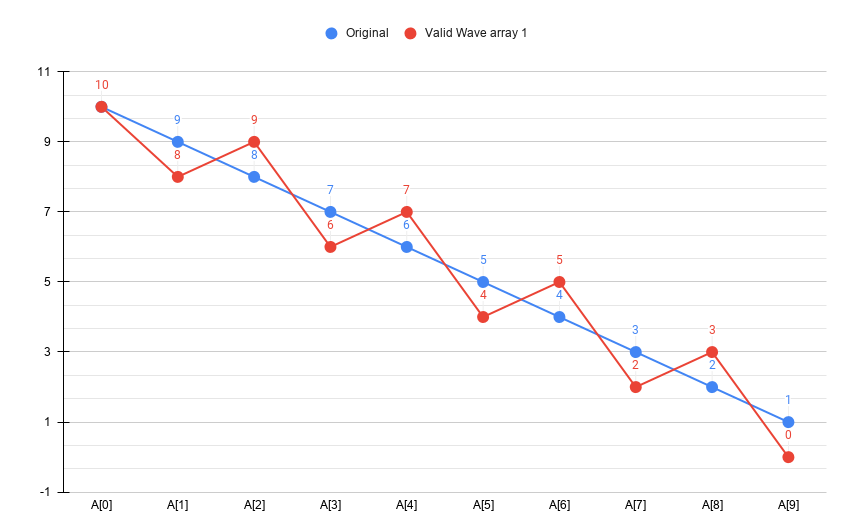
\includegraphics[width=1\linewidth]{sources/wave_array/images/example3.png}
		 \caption{Input and solutions for Example \ref{ex:wave_array:example3}.}
		 \label{fig:wave_array:example13}
	  \end{subfigure}
\end{figure}


\section{Clarification Questions}

\begin{QandA}
	\item \begin{questionitem} \begin{question} Does the array $A$ only contain positive numbers?  \end{question} 	 
    \begin{answered}
		\textit{No, the input numbers can be positive or negative.}
	\end{answered} \end{questionitem}
	\item \begin{questionitem} \begin{question} Are duplicates in $A$ allowed?  \end{question} 	 
    \begin{answered}
		\textit{Yes, duplicates might be present.}
	\end{answered} \end{questionitem}
	\item \begin{questionitem} \begin{question} Do the numbers in $A$ lie in a given particular range? If yes which one?  \end{question} 	 
    \begin{answered}
		\textit{No; no assumptions can be made on the values in $A$.}
	\end{answered} \end{questionitem}
\end{QandA}

\section{Discussion}
\label{wave_array:sec:discussion}
The challenge confronting us here is the creation of an entirely new array $X$ (we, therefore, know from the very beginning we must make a copy of $A$ at some point) that contains the same elements in $A$, arranged in a form that reminds a wave. 
An array of this type has its elements arranged so that they produce a zig-zig-like pattern when plotted on a graph. 

Sequences of numbers of this type can be described as having the property that all of their elements located at even indices are \textbf{all} either 
\textit{local}  \textbf{minima} or  \textbf{maxima}\footnote{An element is a local minimum/maximum if it is lower/higher than its two immediate neighbors.}. 
Identifying a local minimum/maximum is easy but it is only helpful when we want to test whether a sequence is a valid wave array.

\subsection{Brute-force}
\label{wave_array:sec:bruteforce}
One way to attack this problem is by enumerating every possible arrangement of the elements of $A$ and applying the criteria of wave-array validity discussed above to find a solution. 
We can enumerate all permutations of an array quite easily by using a function like \inline{std::next_permutation(Iterator first, Iterator last)} which (taken from the docs): \quoteblock{"Rearranges the elements in the range [first,last) into the next lexicographically greater permutation".}

This idea is implemented in Listing \ref{list:wave_array_linear_bruteforce}.

\lstinputlisting[language=c++, caption=Brute-force time solution to the wave array problem.,label=list:wave_array_linear_bruteforce]{sources/wave_array/wave_array_solution3.cpp}

The code above has a time complexity that is proportional to $n!$ and it is, therefore, impractical to use even for smaller sized arrays as the factorial of $10$ is already greater than $3$ million. 

\subsection{Sorting}
\label{wave_array:sec:sorting}
As per all array problems, the first thing to consider is: \textit{does sorting the elements (we are referring here to a canonical sorting in increasing order) change the difficulty of the problem?}
Incrementally sorted sequences are simpler to approach as they provide strong and clear guarantees on how elements relate to each other. More importantly, the same problem is very often easier to solve on a sorted collection than on an unsorted one.
 
If we apply the wave-array validity criterion (discussed above on local minima/maxima) on a sorted array $S=\{s_0 \leq s_1 \leq \ldots \leq s_{n-1}\}$ we notice that $S$ fails the test as there is only one local minimum and local maximum i.e. $s_0$ and $s_{n-1}$ (which also happen to be the global minimum and maximum).

The question is then how does $S$ change if every element that is located at an even index is swapped with its subsequent neighbor?
When all elements at indices $2i$ and $2i+1$ ($i=0,1,\ldots$) are swapped, then:
$S=\{s_1 \geq s_0 \leq s_3 \geq s_2 \leq s_5 \geq s_4 \leq s_7  \geq \ldots\}$ which is now in better shape to pass the wave-array validity test as every element at even index is surrounded by smaller (or equal) elements. 

Notice that the elements of $S$ have been shuffled around and that the element $a_i$ is not located at index $i$ anymore (contrary to its original position).
We can see that $a_3$ is now located at index $2$ and  is surrounded by $a_0$ and $a_2$, which are both smaller or equal to $a_3$.
Similarly, $a_5$ is now placed at index $4$ and is surrounded by the elements $a_2$ and $a_4$, both known to be smaller or equal than $a_5$.

We can use this observation to solve the problem efficiently and elegantly as shown in  Listing \ref{list:wave_array_sorting}.

\lstinputlisting[language=c++, caption=Solution to the wave array problem using sorting.,label=list:wave_array_sorting]{sources/wave_array/wave_array_solution1.cpp}

Solution \ref{list:wave_array_sorting} works by creating a copy of the input array $A$ named $B$, which is subsequently sorted. The code then proceeds to swap every element located at an even location with the element after it. 
You can see the \inline{swap} operation is applied to the iterators \inline{it} and \inline{it+1}, and that at the end of each iteration \inline{it} is incremented by $2$.
This, together with the fact \inline{it} initially pointer to the first even element at location $0$,  means that only pairs of items at indices of the form $(2i, 2i+1)$ are swapped.

This solution is considered good as its time and space complexity are $O(nlog(n))$
and $O(n)$ respectively.

Before proceeding with this option, it is worth noting that, should the interviewer ask you to return the lexicographical minimum arrangement amongst all possible arrangements, a Brute Force sorting solution  won't work. In such cases you should consider the solutions proposed at section [FILL THIS IN] instead. 


\subsection{Linear time solution}


Although the solution using sorting presented in Section \ref{wave_array:sec:sorting} is likely sufficient for the interview, there is also a solution that works in linear time and that is as easy to
implement and explain. The core idea remains the same: elements at even index should always be
greater (or smaller, equivalently) than their adjacent neighbors. The difference here is that, on this ocassion,  we will enforce it in a single pass on the array by
swapping elements at even indices with their direct neighbors (to the left and to the right) if they happen to be smaller in such a way that the largest element among  $x_{2i-1},x_{2i},x_{2i+1}$ always ends up going to the location $2i$.

We to this by iterating over all even indices and performing the following operations:
\begin{enumerate}
	\item if the current element $a_{2i}$ is smaller than the element $a_{2i-1}$ then swap them; 
	\item if the current element $a_{2i}$ (possibly newly assigned from the previous step) is smaller than the element $a_{2i+1}$ then swap them.
\end{enumerate}
At this point we have effectively placed the largest among $x_{2i-1},x_{2i},x_{2i+1}$ at the location $2i$ and we can proceed to the next even element $a_{2(i+1)}$. 

See Listing \ref{list:wave_array_linear} for a possible implementation of this idea.

\lstinputlisting[language=c++, caption=Linear time solution to the wave array problem.,label=list:wave_array_linear]{sources/wave_array/wave_array_solution2.cpp}

Note that the code above performs some checks on the corner elements so that we do not perform out-of-bound accesses.
This solution is optimal as it runs in $o(n)$ space and time. 

As with the Brute Force sorting solution above unfortunately, the linear time solution also does not work when the lexicographical minimum arrangement should be returned so we will address this common variation now. 

\section{Common Variations - Return the lexicographically smallest}
\label{sec:wave-array:smallest}

One of the most common variations of this problem is the one where you are required to return the lexicographically minimum wave-like arrangement of $A$. In this exercise, you have the chance to apply everything we have learned about this problem so far and write an efficient solution for this variation.

\subsection{Problem statement}
\begin{exercise}
Given an array $A$ of $n$ integers, arrange the numbers in a wave-like fashion (see Section \ref{ex:wave_array:statement} for a definition of wave-array).
If there are multiple valid answers, the function returns the one that is lexicographically smallest.
	\begin{enumerate}
		\item  $x_0 \geq x_1 \leq x_2 \geq x_3 \leq  x_5 \geq \ldots$ where $x_{2i-1} \geq x_{2i} \leq x_{2i+1}$
		\item  $x_1 \leq x_2 \geq x_3 \leq x_4 \geq x_5 \leq \ldots$ where $x_{2i-1} \leq x_{2i} \geq x_{2i+1}$
	\end{enumerate}


	\begin{example}
		\hfill \\
		\label{ex:wave_array:var1:example1}
		Given $A=\{1, 2, 3, 4\}$ the function returns \{2, 1, 4, 3\}. Notice that the sequence \{4, 1, 3, 2\} is also a valid wave-array but it is not lexicographically minimal.
	\end{example}
\end{exercise}

\section{Conclusions}